% Chapter 4

\chapter{Results} % Chapter title

\label{ch:results} % For referencing the chapter elsewhere, use \autoref{ch:results}

%TC:ignore
%Results chapter should be approximately 2,000 Words in total.
%PUF section should be approximately 450 words long.
%Fuzzy Extractor section, it should be approximately 450 words long.
%Cryptographic Hashing section, it should be about 450 words long.
%Networking section, again, it should be 450 words in length.
%Summing up section, it should be 200 words long.
%TC:endignore
%-------------------------------------------------------------------------------

\section{SRAM-PUF}

In testing on various boards the extracted memory was found to exhibit large
differences in output given the same challenge, hence it c
ould informally be seen that there is a large \emph{inter-distance}.
Contrastingly, very little change was ever detected on any one single board
given multiple identical challenges, hence, informally, it would seem that
there is a small \emph{intra-distance}. The purpose of this project is
not to explore the performance of the IS61LV25616 \gls{sram} chip, so this was
not systematically tested, but it is reassuring to know that the chip had the
desired performance characteristics.

While the design was simulated in Mentor Graphic's Modelsim application using a testbench
during initial development, once
minimal functionality was achieved outside simulation the testbench was no longer
used. After further development of the system the testbench code no longer matches
with the implementation and so was deprecated and the earlier waveforms produced
are not included in this dissertation as they are no longer relevant.

The SRAM-PUF was extensively tested simply by connecting the serial cable to a
PC running a common serial terminal emulator. It was found to function well when
data was manually typed by a user, producing the correct 4 digits of hexadecimal
output (the memory contents of an \gls{sram} address) each time 4 corresponding hexadecimal digits
were entered (the memory address of \gls{sram} to select for output).

Timing issues were found to occur when data was sent automatically, either through
\matlab serial functions or through a line-oriented terminal mode. These were
mostly corrected, but issues still occurred when using different setups, lack of time
meant that these issues were never completely eliminated. The SignalTap application
was used to try and detect the source of the issues, but a lack of understanding
of its functionality meant that triggering never occurred correctly and the
investigation proved unfortunately fruitless. It is certain that more work is
required to bring this component up to the sought level of functionality, but
its ability to function manually was sufficient to complete the objectives of the
project.

\section{Fuzzy Extractor}

The results from the fuzzy extractor show that it functions correctly. Below is
a printout from a \matlab which demonstrates the fuzzy extractor running
eleven times. The first run (w) is the generator process providing the original
response (R) and the helper data (s and x). The next seven runs (wa05 - wa15)
are simulated reproduction runs wherein 5, 8, 9, 10 11, 12 and 15 errors are
introduced into the raw response. The last three (wr1 - wr3) simulate the
reproduction runs on non-authentic devices with different randomly generated
raw responses. Next the corresponding responses are given (R00-R15 \& RR1-RR3)
and the simulation concludes with the validation checking which shows that
up to ten errors can be mitigated. It also shows that when a raw response has a
hamming distance from the original greater than 10 the given digest response of
the fuzzy extractor has a hamming distance close to 50\%, i.e. the avalanche
effect of the cryptographic hash in the privacy amplification procedure is
effective in securing the response and preventing replay attacks:

\begin{verbatim}
w = D9DA7BEA1A31D8ABE2A27B4E855C5C5C
wa05 = D9DA6BEA1B31D8A3E2A27B4E857C5E5C
wa08 = D1D27BEA3A21D8ABE2A27B4E955D545E
wa09 = F9CA7BE21A71D8ABE2C27B4E855CDDDC
wa10 = DBEA7BCA1E21F8ABE2B27B4CA55C5C5C
wa11 = D0DA7BA81CB0D8ABE2E23B6E855C5C5C
wa12 = D1DA7BEA1A35DCBBE6B37B4AA15DDC5C
wa15 = D8DBFBEA5AB580ABE2B27B2E815C4C5E
wr1 = 7B86B5F833E9BF6A0EE6538261C5A7AE
wr2 = DD4DC9E1AAD2BB30051F0F6F2E1CB7F9
wr3 = BBD3AE3E9D8B3CE8867A027F0979F8F6

R = 5204AD19BDFA759B36D1CEF842B924C15A977F112E246CC4A5336E149058BDE6
s = 35B5595F99E4A446741CAFEE3F1C08C4
x = 37982001400E20B7A67AB050F073F429

R00 = 5204AD19BDFA759B36D1CEF842B924C15A977F112E246CC4A5336E149058BDE6
R05 = 5204AD19BDFA759B36D1CEF842B924C15A977F112E246CC4A5336E149058BDE6
R08 = 5204AD19BDFA759B36D1CEF842B924C15A977F112E246CC4A5336E149058BDE6
R09 = 5204AD19BDFA759B36D1CEF842B924C15A977F112E246CC4A5336E149058BDE6
R10 = 5204AD19BDFA759B36D1CEF842B924C15A977F112E246CC4A5336E149058BDE6
R11 = CB3B16EFADAB739429A5381A5F9C21E112D23487E933B0A7B6FCA4BDF4809B99
R12 = B01F5CFF14677D560D1CEBD5C876A458BA761B563622CD4C1413690454E8464F
R15 = 5225B4E08066191C29395423B0DCDA8F4B4C4DFB73CD254B1F57CAE5DD455E13
RR1 = 23DA1F0810BD6D6D73C1C61E659267F2132DF43BB729D1702A53944F754E941A
RR2 = DF0BC75A7A5D346B4E67FDD1A4CC67C0807E4ABFFD3F90A5BFDD70689B623B5D
RR3 = 43737B59470BFBA2056FD47B239536389EDAFF3B3AAA2FDBD63D8472269FA7D1

The R00 device passed verification
The R05 device passed verification
The R08 device passed verification
The R09 device passed verification
The R10 device passed verification
The R11 device failed verification, distance: 49.2%
The R12 device failed verification, distance: 44.1%
The R15 device failed verification, distance: 53.1%
The RR1 device failed verification, distance: 48.8%
The RR2 device failed verification, distance: 51.6%
The RR3 device failed verification, distance: 48.0%
\end{verbatim}

Next the ability to alter attributes of the fuzzy extractor is shown. The test
is the same, but this time the SRAM-PUF data width is halved to 64 bits and the
message length is correspondingly reduced to 30 bits. Thus only 6 bits can be
corrected. The output shown the fuzzy extractor performing accordingly:

\begin{verbatim}
w = 673E9620164BD71E
wa04 = 633E9660164BF71F
wa05 = 673A12201249D71E
wa06 = 672A8660364BD79E
wa07 = 6736DEA0024BD31E
wr1 = 410BCBA3D7C877AE
wr2 = 9B05581D6F8CEC6C
wr3 = F3BB6A432F7D979F

R = 3DAD18154B7010A439AA68448151F61E74A727229DB50D8576AC59EF2F353C81
s = 3C7F8142BE595539
x = 390F18C57D17BB8E

R00 = 3DAD18154B7010A439AA68448151F61E74A727229DB50D8576AC59EF2F353C81
R04 = 3DAD18154B7010A439AA68448151F61E74A727229DB50D8576AC59EF2F353C81
R05 = 3DAD18154B7010A439AA68448151F61E74A727229DB50D8576AC59EF2F353C81
R06 = 3DAD18154B7010A439AA68448151F61E74A727229DB50D8576AC59EF2F353C81
R07 = 741373A3B67B00242E02F0EE90D07A47C08DAB741086D39F7C0D46DF8CF37C71
RR1 = 0F1069EB2913962B55B410EA144BDC594AC97BA8A33CA94EA789FA539348A0BD
RR2 = 5A28A8EB40D64B96730CB9A45D26B0019EFAC0ECD0A09ABF4A994BD7349AEBB2
RR3 = 39B7AC78B67FEBA7C20273E24F178DB9B68985B16B22D621914B1D524F54CD60

The R00 device passed verification
The R04 device passed verification
The R05 device passed verification
The R06 device passed verification
The R07 device failed verification, distance: 43.8%
The RR1 device failed verification, distance: 52.3%
The RR2 device failed verification, distance: 53.1%
The RR3 device failed verification, distance: 53.9%
\end{verbatim}

\section{SHA-256}

The sha-256 implementation was tested to ensure it conformed with the standard
specification given in \cite{fips2001180} exactly. It was tested against the
worked example included in an official description document\cite{shsnist} and
implementations available on the web and iPhone apps. It was shown to follow
the specification exactly, as long as the message fits into one block.

The output generated from \matlab when running the implementation of SHA-256
against the hexadecimal encoding of the \gls{ascii} text `abc':

\begin{verbatim}
>> sha256('616263')
ans = BA7816BF8F01CFEA414140DE5DAE2223B00361A396177A9CB410FF61F20015AD
\end{verbatim}

This can be seen to be the same result as that given on page 11 of \cite{shsnist}.

\section{Ethernet Authentication}

Code to simulate the generation and extraction of data from Ethernet packets
with EAP-PUF protocol bodies were developed (see \autoref{app:eappuf}). The
resulting hexadecimal packets were constructed as follows:

\begin{description}
\item[EAPoL Start Packet (From Supplicant)] \hfill \\
\inlinecode{0180C200000300005E005301888E02010000} + 4 Byte CRC
\item[EAP Identity Request Packet (From Authenticator)] \hfill \\
\inlinecode{00005E00530100005E0053FF888E020000060155000601B0} + 4 Byte CRC
\item[EAP Identity Response Packet (From Supplicant)] \hfill \\
\inlinecode{00005E0053FF00005E005301888E0200000B0255000B0100005E005301} + 4 Byte CRC
\item[EAP EAP-PUF Request Packet (From Authenticator)] \hfill \\
\inlinecode{00005E00530100005E0053FF888E0200003501550035B0} + Challenge(16 Bytes)
                                               + Helper Data(32 Bytes)
                                               + 4 Byte CRC
\item[EAP EAP-PUF Response Packet (From Supplicant)] \hfill \\
\inlinecode{00005E0053FF00005E005301888E0200002502550025B0} + Response(32 Bytes)
                                               + 4 Byte CRC
\item[EAP Success Packet (From Authenticator)] \hfill \\
\inlinecode{00005E00530100005E0053FF888E0200000403550004} + 4 Byte CRC
\item[EAPoL Logoff Packet (From Supplicant)] \hfill \\
\inlinecode{0180C200000300005E005301888E02020000} + 4 Byte CRC
\end{description}

These Ethernet packet stubs have been checked and verified to correctly follow
the specification proposed.

\subsection{CRC}

The \gls{crc} algorithm is used to generate the \gls{fcs} appended to every
Ethernet packet. Below is the output of running the \matlab implementation
developed for this project against the EAPoL Start Packet as generated above:

\begin{verbatim}
>> crc('0180C200000300005E005301888E02010000')
ans = F7D19377
\end{verbatim}

This can be seen to be the same as the specification by checking using the online
\gls{fcs} generator at \inlinecode{http://www.lammertbies.nl/comm/info/crc-calculation.html}.

\section{Overall System Results}

The overall system was tested through a demonstration as shown in \autoref{fig:demo}.
While not all parts of the EAP-PUF protocol were simulated and there are still
issues with the \gls{uart} implementation in communicating effectively with \matlab,
in general terms the system can be said to be functional in a prototype form.

There is much that could be done to improve and develop the implementation, but
it shows in broad terms that the design proposed works, which was the intention
of the project.

\begin{figure}
  \centering
  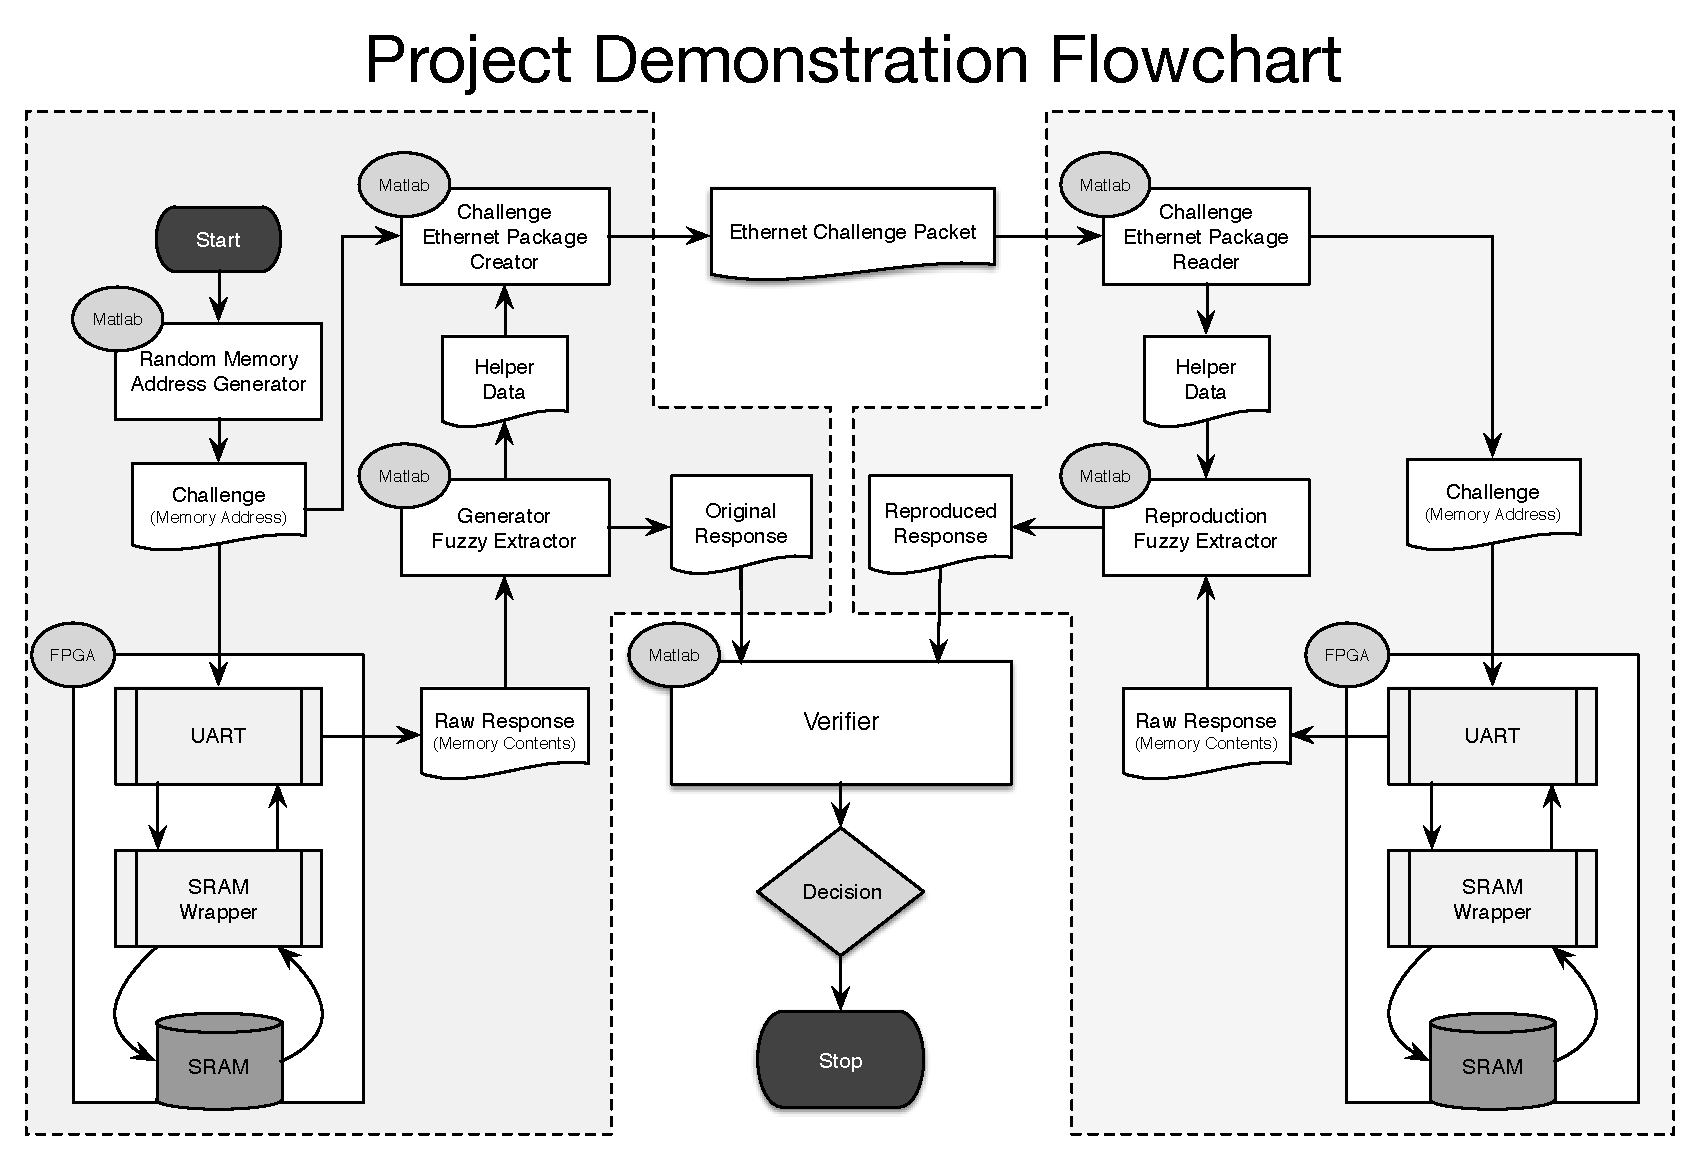
\includegraphics[angle=270, scale=0.8]{images/flowchart}
  \caption{Full system testing demonstration flowchart}
  \label{fig:demo}
\end{figure}
